\documentclass[12pt]{article}

% --- 1. 基础宏包配置 ---
\usepackage[a4paper, margin=0.8cm, portrait]{geometry}
\usepackage[utf8]{inputenc}
\usepackage{tikz}
\usetikzlibrary{shapes.geometric, arrows.meta, calc}
\usepackage{adjustbox}
\usepackage{xcolor}
\usepackage{anyfontsize}
\usepackage{sfmath}

\renewcommand{\familydefault}{\sfdefault}

% --- 2. 全局参数与颜色定义 (基于 2001-02-28 出生计算) ---
\def\myAge{24}            
\def\myWeek{43}           
\def\myMonth{298}         

\definecolor{textDarkBlue}{HTML}{000080}
\definecolor{textOrange}{HTML}{D9730D}
\definecolor{annotationPurple}{HTML}{802080}
\definecolor{annotationBlue}{HTML}{0000FF}
\definecolor{weekFill}{HTML}{F26522}
\definecolor{monthFill}{HTML}{00A99D}
\definecolor{yearFill}{HTML}{2E3192}

% --- 3. TikZ 样式定义 (统一标准) ---
\tikzset{
    HugeTitle/.style={font=\fontsize{70}{84}\selectfont\bfseries},
    NormalTitle/.style={font=\fontsize{48}{58}\selectfont\bfseries},
    SubHeaderText/.style={font=\fontsize{24}{28}\selectfont\bfseries},
    AxisText/.style={font=\fontsize{26}{32}\selectfont\bfseries},
    BirthStyle/.style={font=\fontsize{28}{34}\selectfont\bfseries, text=annotationBlue},
    TurningStyle/.style={font=\fontsize{28}{34}\selectfont\bfseries, text=annotationPurple},
    OtherNoteStyle/.style={font=\fontsize{22}{26}\selectfont\bfseries, text=black!70},
    LabelArrow/.style={-{Stealth[scale=1.5]}, line width=2pt}
}

\begin{document}
\pagestyle{empty}

% ============================================================
% 第一页:周表 (Weeks) 
% ============================================================
\noindent\begin{adjustbox}{width=\textwidth, height=0.98\textheight, keepaspectratio}
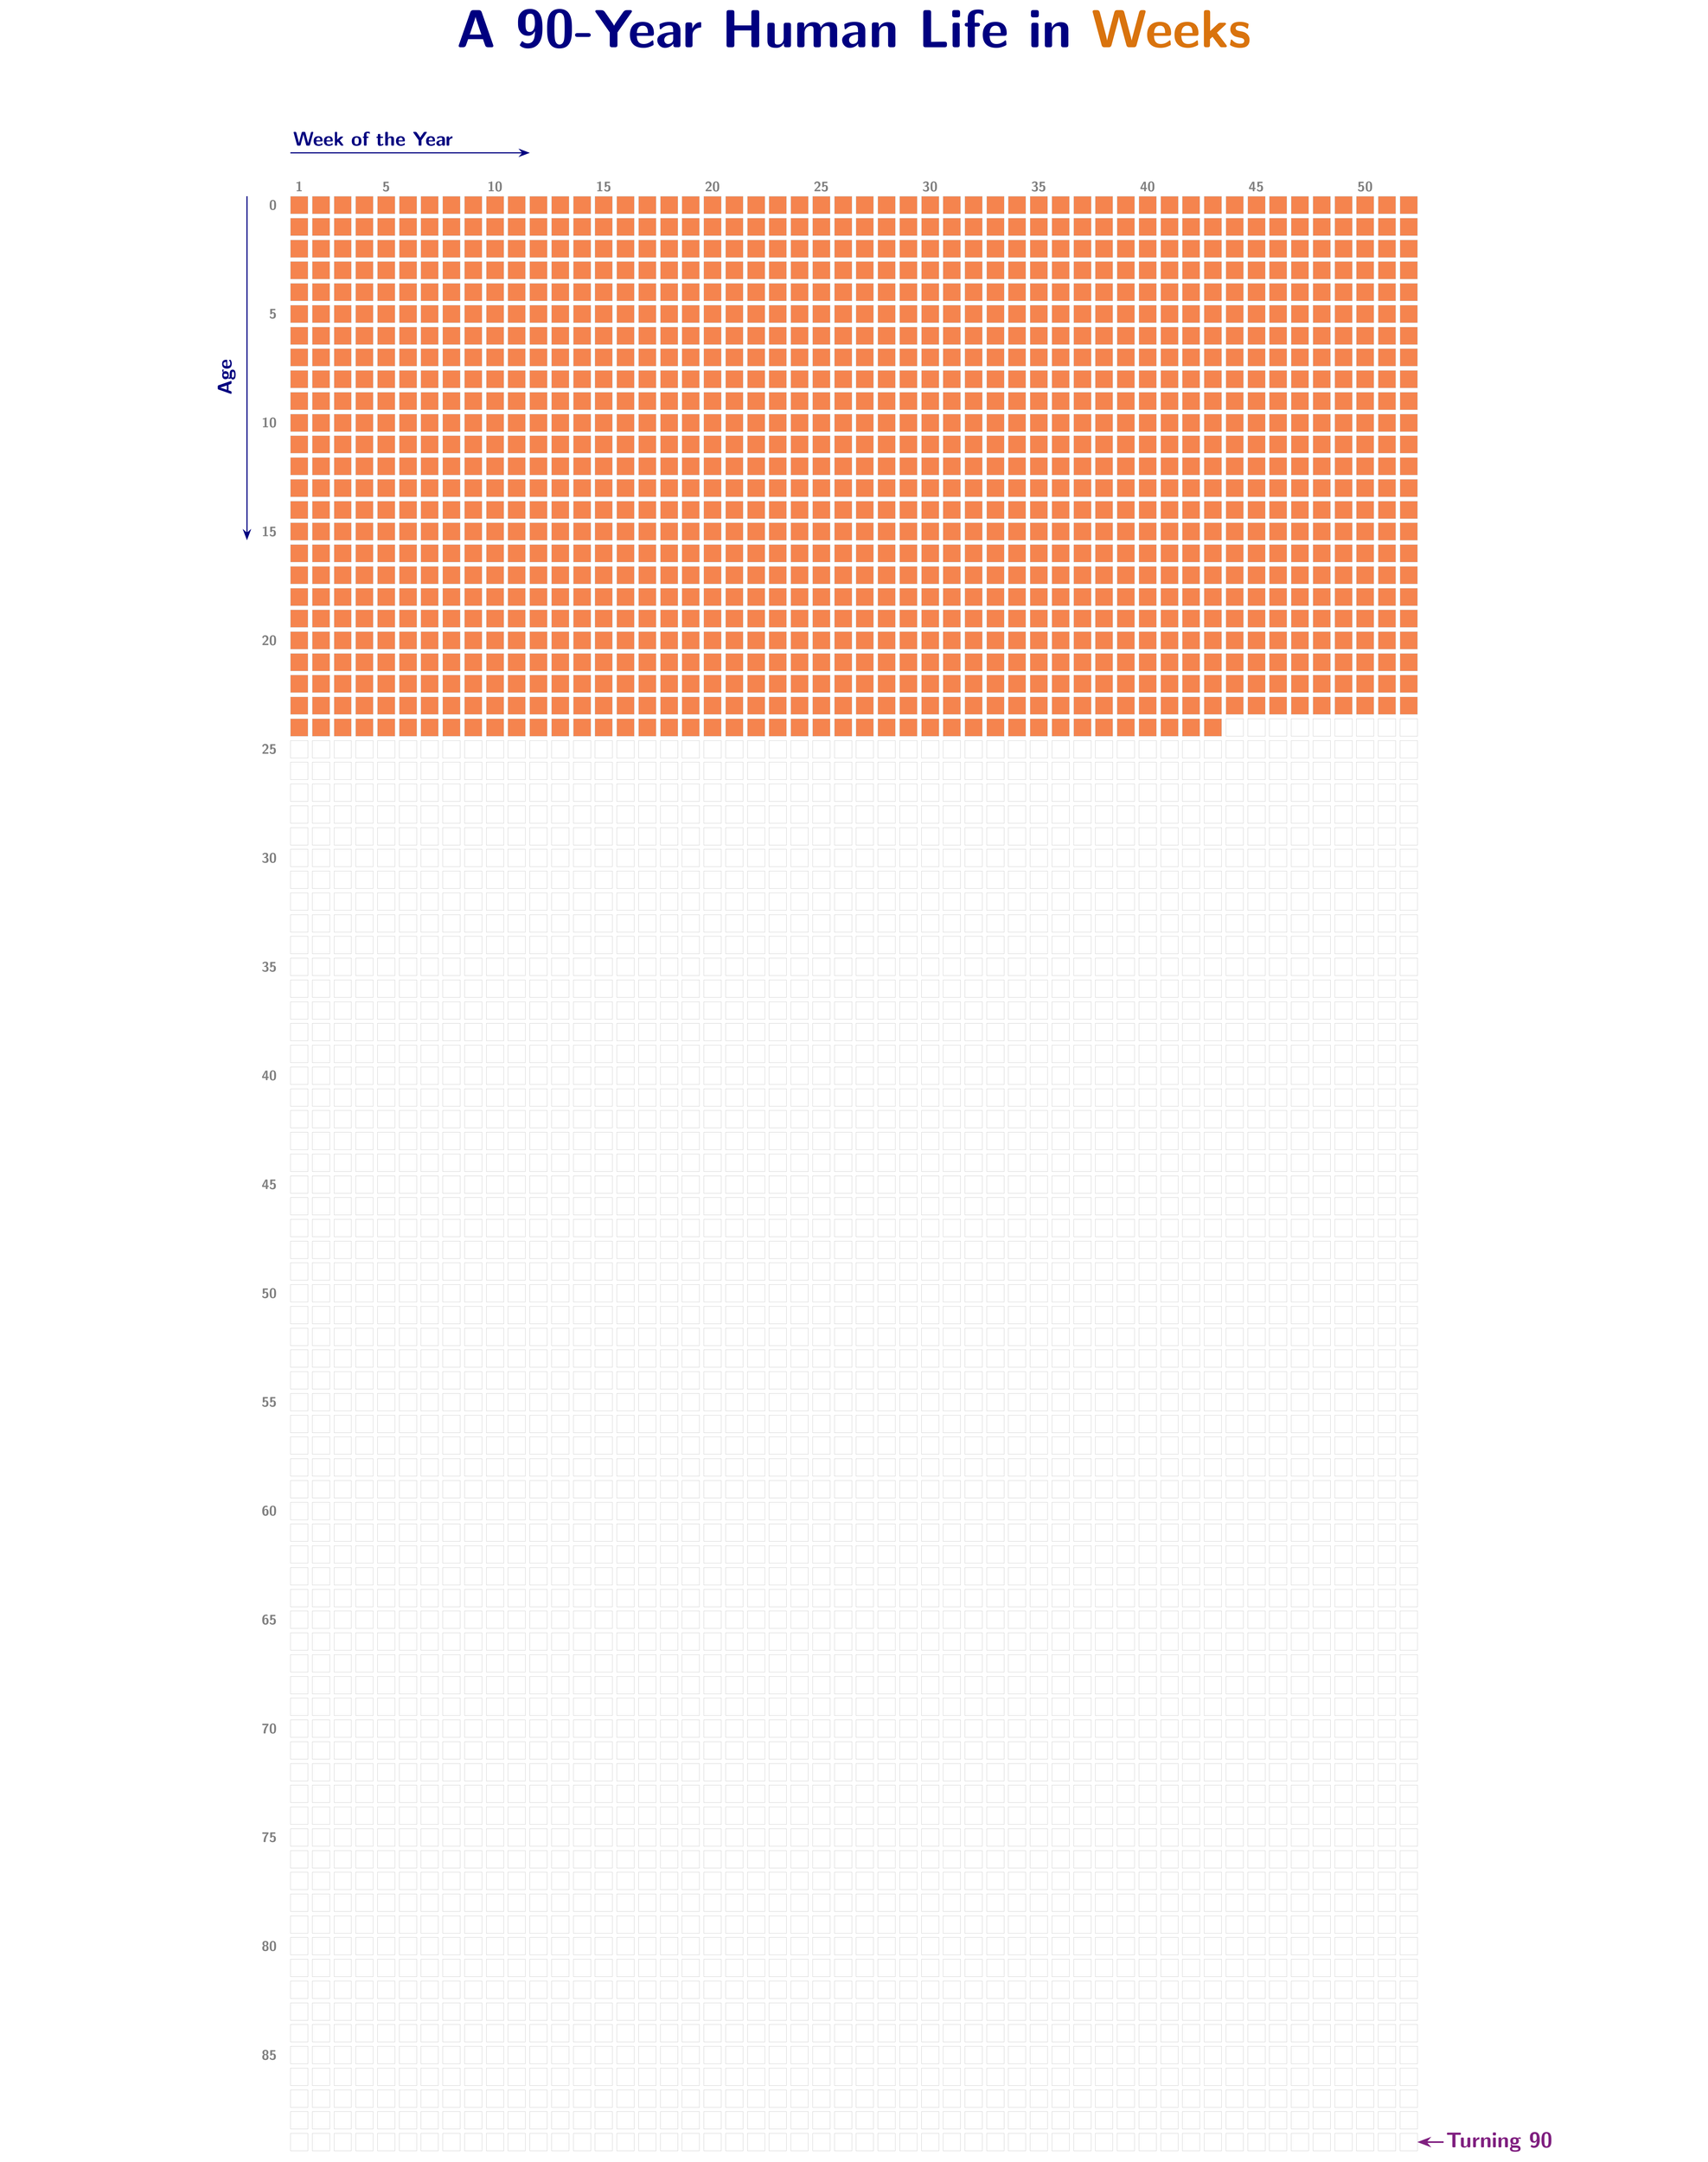
\begin{tikzpicture}[x=1cm, y=1cm]
    % 定义网格中轴线:(起始1 + 结束52.8)/2 = 26.9
    \def\gridCenter{26.9}
    % --- 【修正】轴线间距由 1.2 调大至 2.0,防止 Age 轴线与数字 10 等重叠 ---
    \def\axisGap{2.0} 
    
    % --- 【修正】标题改为居中对齐,确保在视觉中心 ---
    \node[anchor=center, text=textDarkBlue, HugeTitle] at (\gridCenter, 8.5) {A 90-Year Human Life in \textcolor{textOrange}{Weeks}};

    % 顶部 Week of the Year 轴线
    \draw[textDarkBlue, -{Stealth[scale=1.5]}, line width=1.5pt] (1, {0.8+\axisGap}) -- (12, {0.8+\axisGap});
    \node[anchor=south west, text=textDarkBlue, AxisText] at (1, {0.8+\axisGap+0.2}) {Week of the Year};

    % 左侧 Age 轴线
    \draw[textDarkBlue, -{Stealth[scale=1.5]}, line width=1.5pt] ({1-\axisGap}, 0.8) -- ({1-\axisGap}, -15);
    \node[above, rotate=90, text=textDarkBlue, AxisText] at ({1-\axisGap-0.4}, -7.5) {Age};

    % 绘制方格
    \foreach \age in {0,...,89} {
        \ifnum\numexpr\age/5*5=\age\relax
            \node[left, font=\fontsize{18}{22}\selectfont\bfseries, gray] at (0.5, -\age+0.4) {\age};
        \fi
        \foreach \week in {1,...,52} {
            \pgfmathsetmacro{\isFilled}{(\age < \myAge || (\age == \myAge && \week <= \myWeek) ? 1 : 0)}
            \pgfmathsetmacro{\cellFill}{(\isFilled == 1 ? "weekFill!80" : "white")}
            \draw[fill=\cellFill, draw=black!25, line width=0.2pt] (\week, -\age) rectangle ++(0.8, 0.8);
        }
    }
    
    \foreach \w in {1, 5, 10, 15, 20, 25, 30, 35, 40, 45, 50}
        \node[above, font=\fontsize{18}{22}\selectfont\bfseries, gray] at (\w+0.4, 0.9) {\w};

    % 统一标注:周表 Birth & Turning 90
    %\node[BirthStyle, left] (bw) at ({1-\axisGap-0.5}, 0.4) {Birth};
    %\draw[annotationBlue, LabelArrow] (bw.east) -- (0.8, 0.4);

    \node[TurningStyle, right] (tw) at (54, -88.6) {Turning 90};
    \draw[annotationPurple, LabelArrow] (tw.west) -- (52.8, -88.6);

    % --- 【关键】增加对称路径强制页面居中 ---
    % 右侧最远端约在 65.8 (含文字宽度),中轴线 26.9,故左侧补齐至 -12.0
    \path (-12, 0) (65.8, 0); 
\end{tikzpicture}
\end{adjustbox}

\clearpage

% ============================================================
% 第二页:合并月表和年表 (统一风格与间距优化)
% ============================================================
\centering

% --- 2.1 月表 (Months) ---
\noindent\begin{adjustbox}{width=\textwidth, height=0.52\textheight, keepaspectratio}
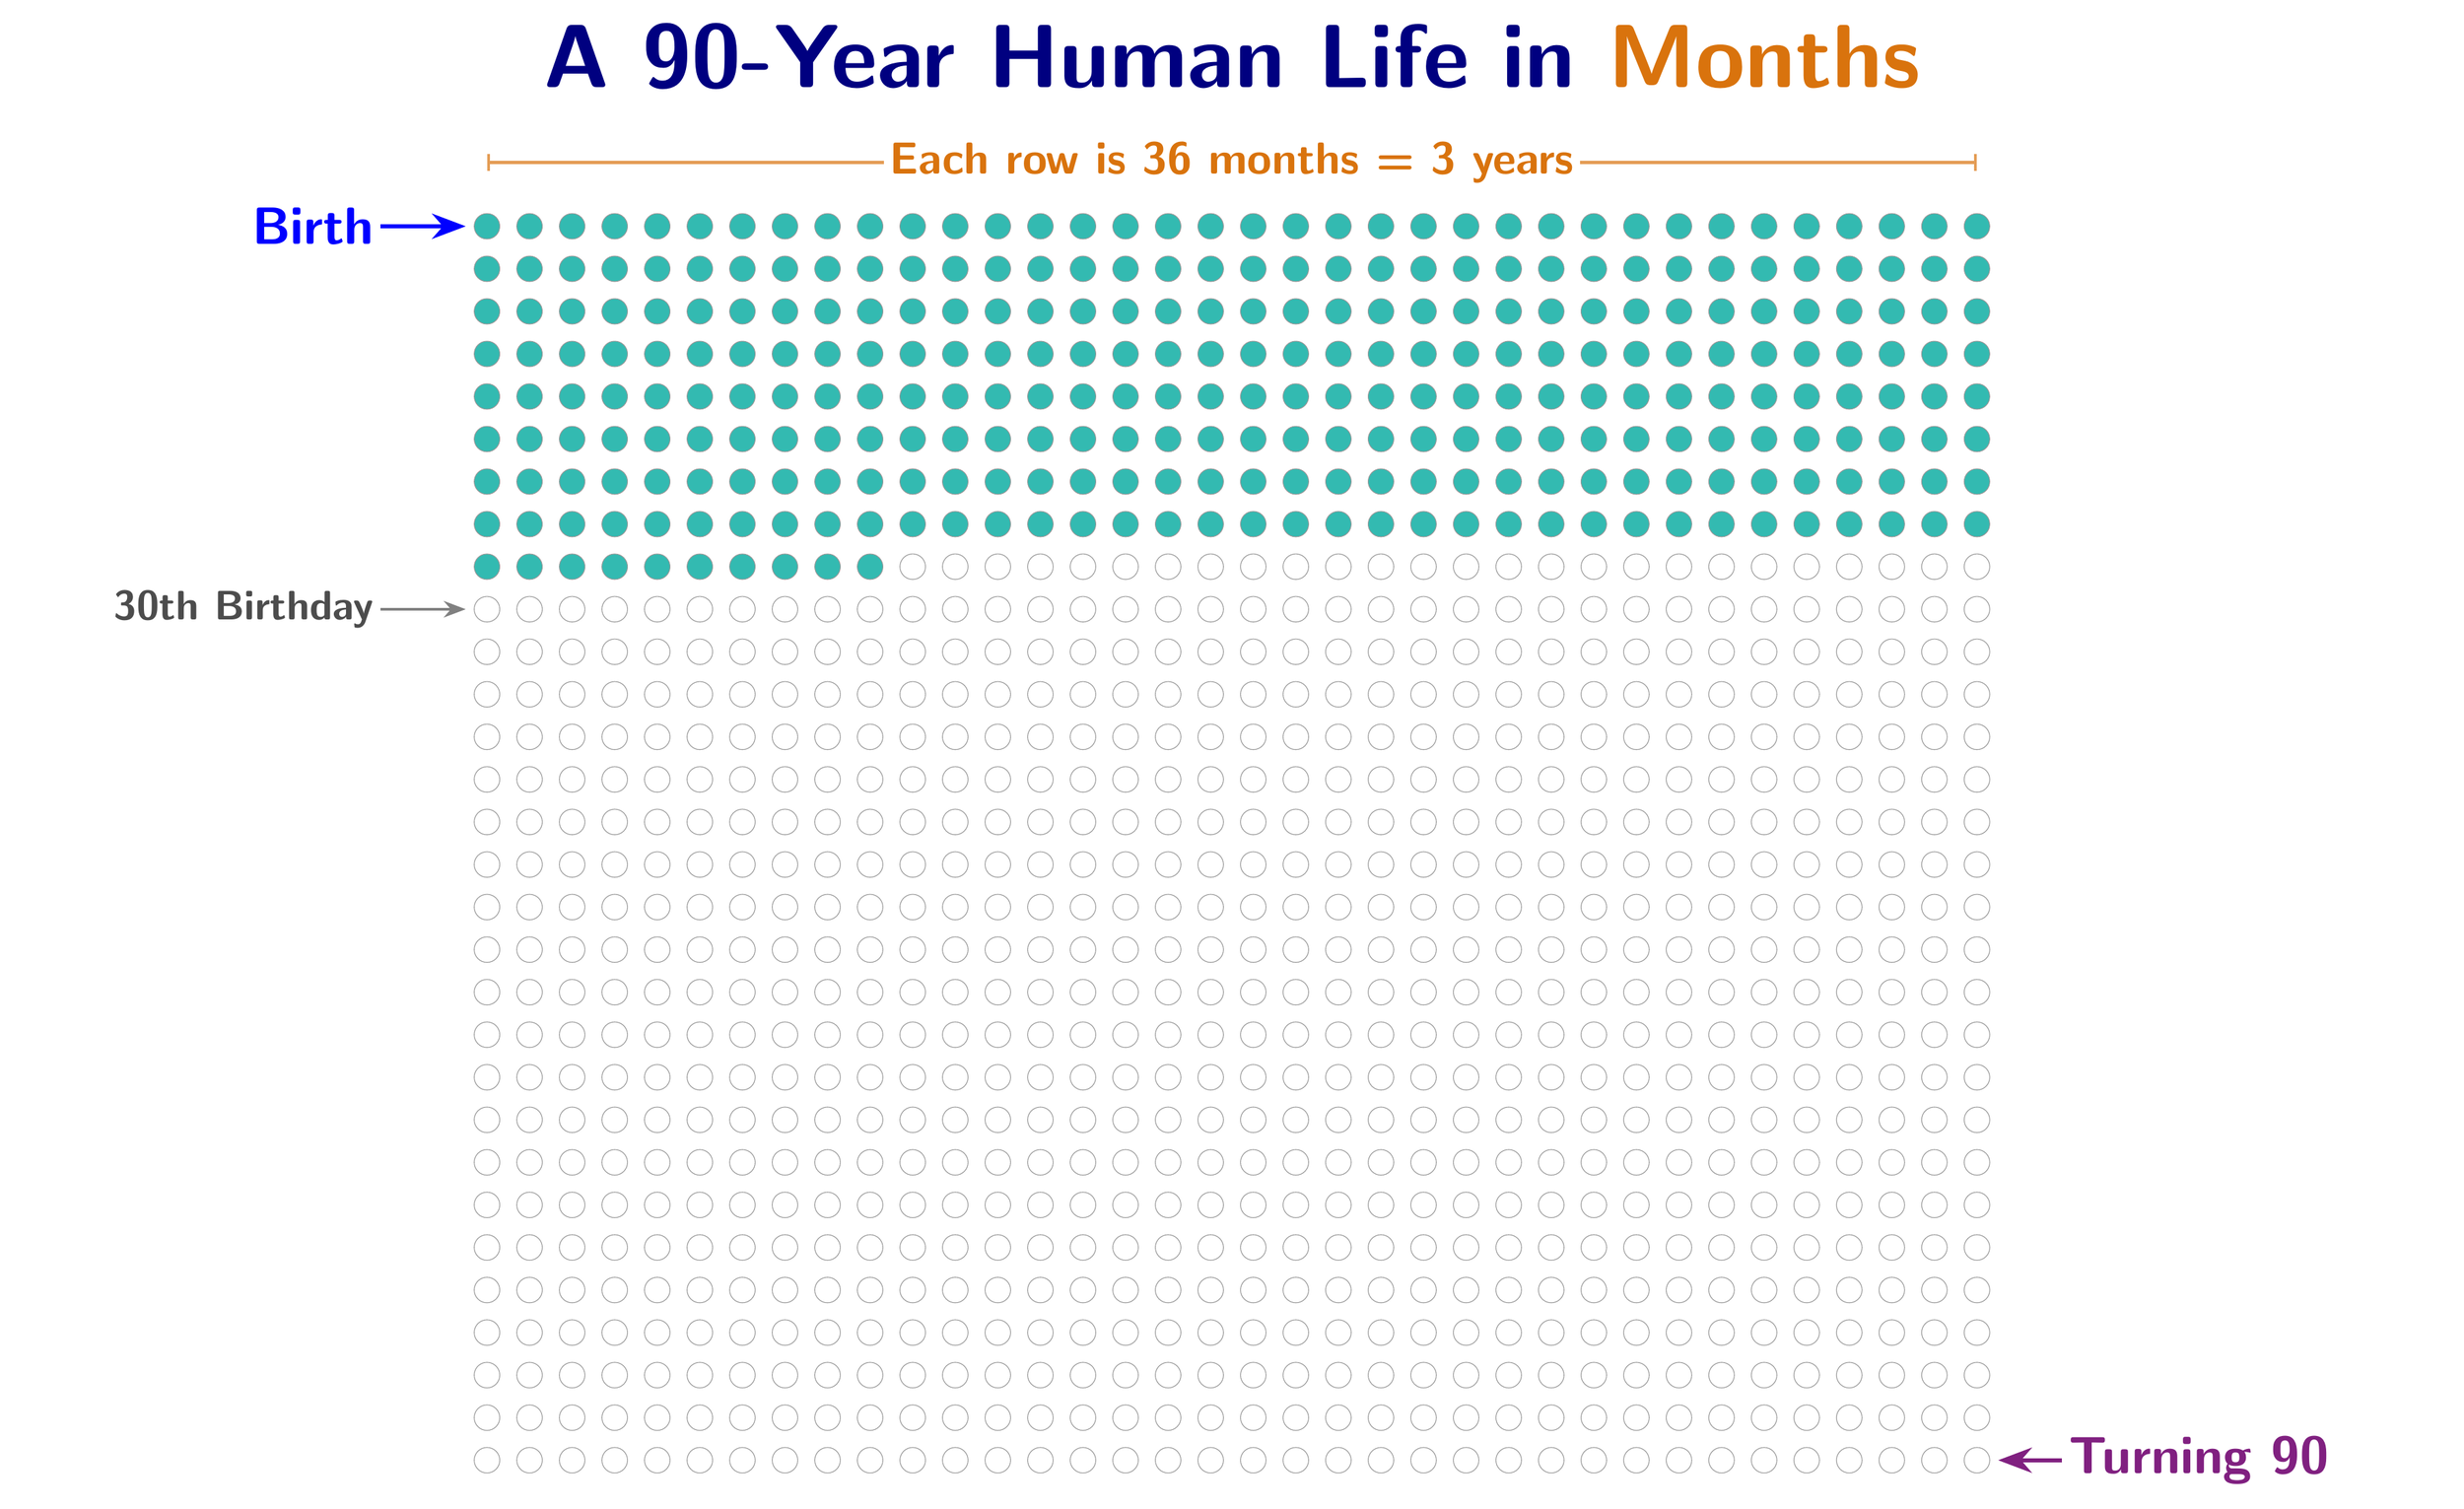
\begin{tikzpicture}[x=0.8cm, y=0.8cm]
    \node[anchor=center, text=textDarkBlue, NormalTitle] at (18.5, 4.0) {A 90-Year Human Life in \textcolor{textOrange}{Months}};
    
    % 比例尺线条下移,更贴近方格
    \draw[textOrange!70, |-| , line width=1.5pt] (1, 1.5) -- (36, 1.5) 
        node[midway, fill=white, text=textOrange, SubHeaderText] {Each row is 36 months = 3 years};

    \foreach \row in {0,...,29} {
        \foreach \col in {1,...,36} {
            \pgfmathsetmacro{\mIndex}{\row * 36 + \col}
            \pgfmathsetmacro{\mFill}{(\mIndex <= \myMonth ? "monthFill!80" : "white")}
            \draw[fill=\mFill, draw=black!40, line width=0.4pt] (\col, -\row) circle (0.3);
        }
    }
    
    % 统一标注:月表
    \node[BirthStyle, left] (bm) at (-1.5, 0) {Birth};
    \draw[annotationBlue, LabelArrow] (bm.east) -- (0.5, 0);

    \node[OtherNoteStyle, left, align=right] (bm30) at (-1.5, -9) {30th Birthday};
    \draw[black!50, -{Stealth[scale=1.2]}, line width=1.5pt] (bm30.east) -- (0.5, -9);

    \node[TurningStyle, right] (tm90) at (38, -29) {Turning 90};
    \draw[annotationPurple, LabelArrow] (tm90.west) -- (36.5, -29);
    
    % 月表补齐中心
    \path (-10, 0) (47, 0);
\end{tikzpicture}
\end{adjustbox}

\vspace{3cm} 

% --- 2.2 年表 (Years) ---
\noindent\begin{adjustbox}{width=\textwidth, height=0.32\textheight, keepaspectratio}
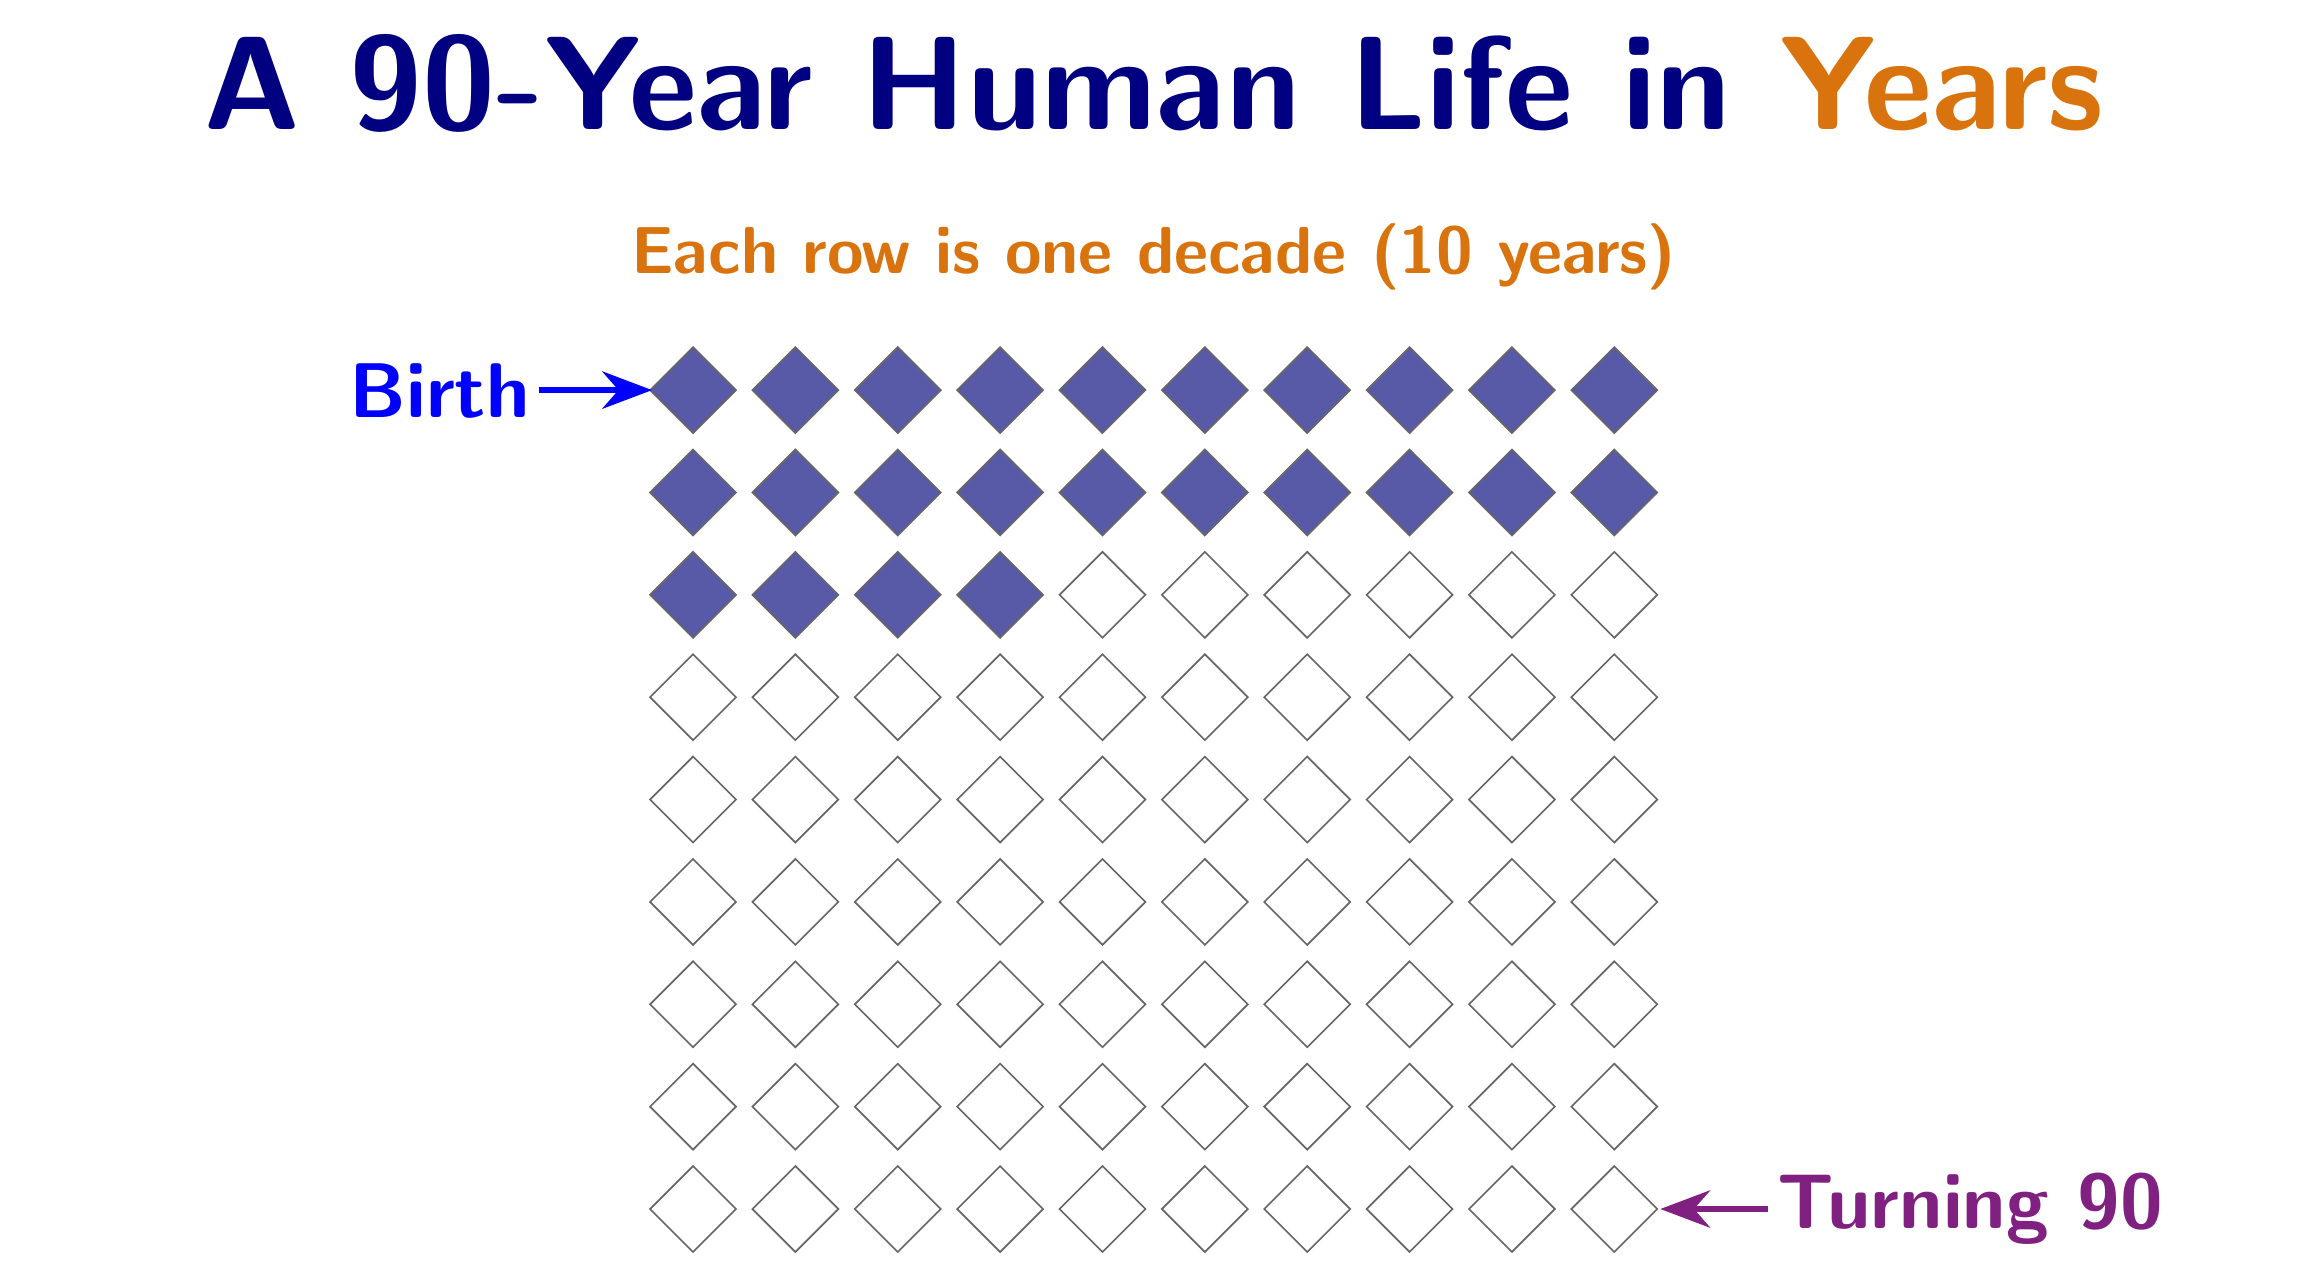
\begin{tikzpicture}[x=1.3cm, y=1.3cm]
    \node[anchor=center, text=textDarkBlue, NormalTitle] at (5.5, 3.0) {A 90-Year Human Life in \textcolor{textOrange}{Years}};
    
    % 比例尺线条风格对齐并下移
    \draw[textOrange!70, |-| , line width=1.5pt] (1, 1.3) -- (10, 1.3) 
        node[midway, fill=white, text=textOrange, SubHeaderText] {Each row is one decade (10 years)};

    \foreach \y in {0,...,8} {
        \foreach \x in {1,...,10} {
            \pgfmathsetmacro{\yFill}{(\y * 10 + \x <= \myAge ? "yearFill!80" : "white")}
            \node[draw=black!60, line width=0.6pt, diamond, minimum size=1.1cm, fill=\yFill] at (\x, -\y) {};
        }
    }
    
    % 统一标注:年表 Birth
    \node[BirthStyle, left] (by) at (-0.5, 0) {Birth};
    \draw[annotationBlue, LabelArrow] (by.east) -- (0.6, 0);

    % 统一标注:年表 Turning 90
    \node[TurningStyle, right] (ty90) at (11.5, -8) {Turning 90};
    \draw[annotationPurple, LabelArrow] (ty90.west) -- (10.45, -8);
    
    \path (-5.5, 0) (16.5, 0); % 强制对称补齐
\end{tikzpicture}
\end{adjustbox}

\end{document}